\documentclass[]{article}

\usepackage{graphicx}
\usepackage{tabularx}

\begin{document}

\section{Naming Conventions}

\subsection{Variable Naming Conventions}

\begin{itemize}
\item Component names should be capitalised e.g OVEN
\item The first letter of a behavior should be captialised e.g Open
\item The first letter of an attribute should be lowercase e.g. timer
\end{itemize}

\begin{table}
\begin{tabularx}{\textwidth}{|c|X|}
\textbf{Variable} & \textbf{Description}\\ \hline
$N,N_i$ & Behavior Tree Nodes\\ \hline
$T,T_i$ & Behavior Trees\\ \hline
$C,C_i$ & Components\\ \hline
$C\#$ & A Component Instance\\ \hline
$s$ & A State of a Component\\ \hline
$e$ & An Event\\ \hline
$a$ & An Attribute of a Component\\ \hline
$b$ & A Branching Condition of a Component
\end{tabularx}
\caption{Variable Naming Conventions}
\label{Variable Naming Conventions}
\end{table}

\subsection{Node Naming Conventions}

\begin{table}
\begin{tabularx}{\textwidth}{|c|l|X|}
\textbf{Label} & \textbf{Name} & \textbf{Description}\\ \hline
A & Component Name & Specifies a component\\ \hline
B & Behavior & Specifies the behavior associated with the component\\ \hline
C &Operator & Describes threaded behavior that is linked to the matching node in the tree\\ \hline
D &Label & An optional label for disambiguation (in case a node appears elsewhere with the same component and behavior)\\ \hline
E &Behavior Type & Delimiters on the behavior indicating the type of behavior involved\\ \hline
F & Traceability Link & A reference to the requirements document\\ \hline
G & Traceability Status & Indicates how the node relates to the traceability link\\ \hline
H &Tag & The box on the left-hand side of the node (may be omitted in different contexts)\\ \hline
I & Behavior Tree Node & A node consisting of all or some of the information above
\end{tabularx}


\caption{Elements of a Behavior Tree Node}
\label{tbl:BTNodeElements}
\end{table}

\begin{figure}
 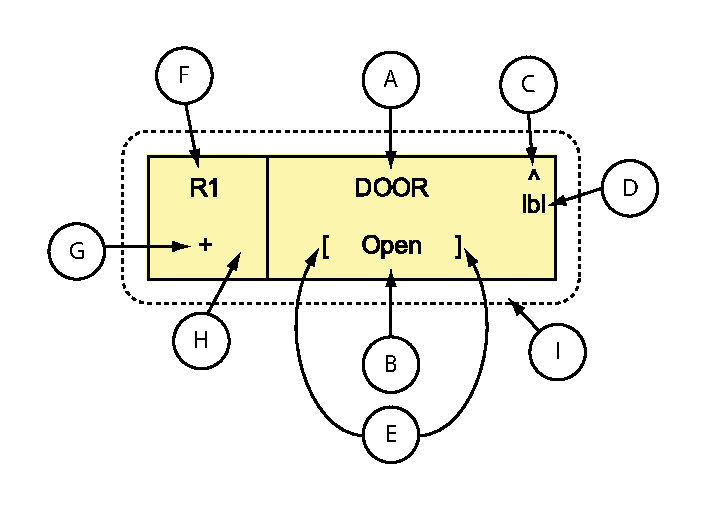
\includegraphics{figs/AppendixB/Naming/Fig1}
 \caption{Behavior Tree Node Naming Conventions}
 \label{fig:Naming1}
\end{figure}

\subsection{Relation Naming Conventions}

\begin{table}
\begin{tabularx}{\textwidth}{|c|l|X|}
 \textbf{Label} & \textbf{Name} & \textbf{Description}\\ \hline
A & Primary Component &The component and behavior that form the relation\\ \hline
& \& Behavior &\\ \hline
B &Related Component & Component (and optional behavior) related to the primary component and behavior\\ \hline
C &Qualifier & Specifies the type of the relation. Must be one of What, Where, When, Why, Who or How\\ \hline
D &Preposition & Further qualifies the relation to remove potential ambiguity\\ \hline
E &Secondary Relation & The related component is linked to the primary component using a forward slash (/). Multi-level relations can be formed by using multiple forward slashes
\end{tabularx}


\caption{Elements of a Behavior Tree Relation}
\label{tbl:RelationElements}
\end{table}

\begin{figure}
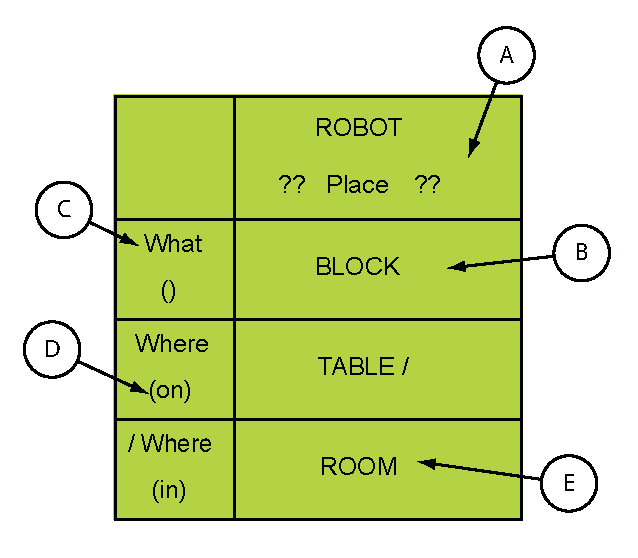
\includegraphics{figs/AppendixB/Naming/Relation}
\caption{Behavior Tree Relation Naming Conventions}
\label{fig:RelationNaming}
\end{figure}

\subsection{Tree Naming Conventions}

\begin{table}
\begin{tabularx}{\textwidth}{|c|l|X|}
\textbf{Label} & \textbf{Name} & \textbf{Description}\\ \hline
A & Ancestor Node & Any node which appears in a direct line between the node of interest and the root node of the tree\\ \hline
B & Parent Node & An immediate ancestor\\ \hline
C & Sibling Node & A node which shares the same parent\\ \hline
D & Sibling Branch & A subtree with a sibling node as its root\\ \hline
E & Child Node & A node immediately below the node of interest\\ \hline
F & Descendant & Any node appearing below the node of interest
\end{tabularx}

\caption{Nodes of a Behavior Tree}
\label{BTTree Nodes}
\end{table}

\begin{figure}
 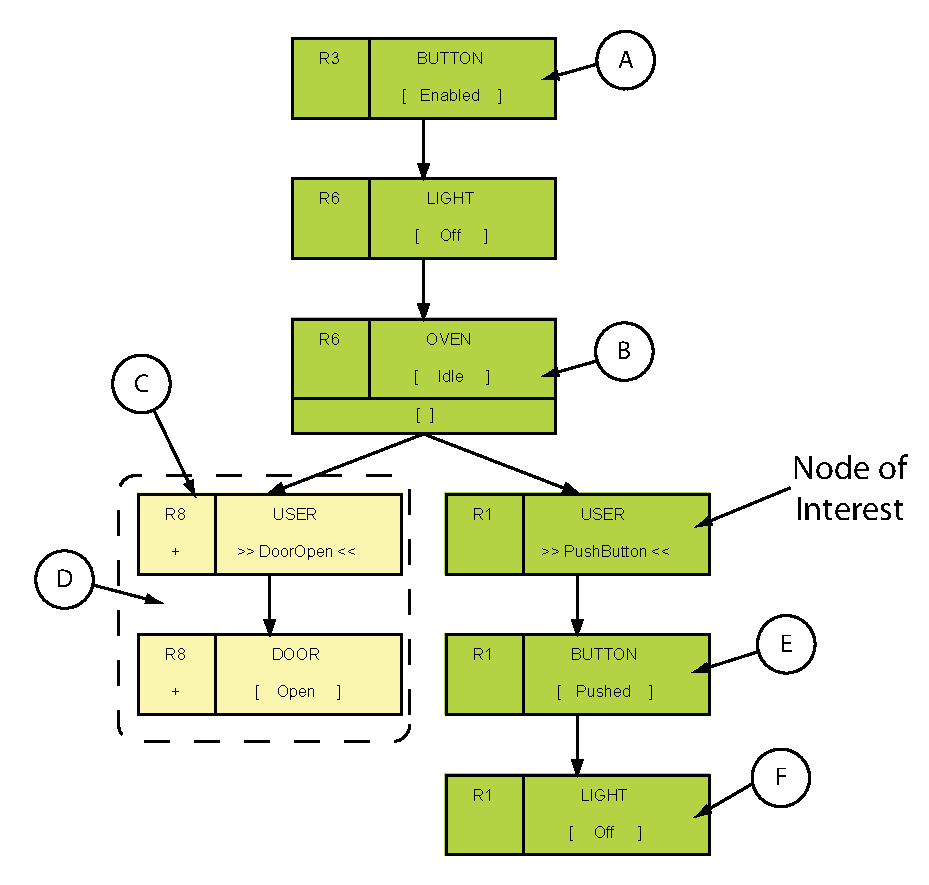
\includegraphics{figs/AppendixB/Naming/Fig2}
 \caption{Behavior Tree Tree Naming Conventions}
 \label{fig:Naming2}
\end{figure}

\subsection{Tree Branch Naming Convention}

\begin{table}
\begin{tabularx}{\textwidth}{|c|l|X|}
 \textbf{Label} & \textbf{Name} & \textbf{Description}\\ \hline
A & Root Node & The first node in a tree (does not have a parent)\\ \hline
B & Edge & A connection between two nodes\\ \hline
C & Leaf Node & A node with no children\\ \hline
D & Branch & A subtree of the node of interest
\end{tabularx}
\caption{Branches of a Behavior Tree}
\label{BTTree Branches}
\end{table}

\begin{figure}
 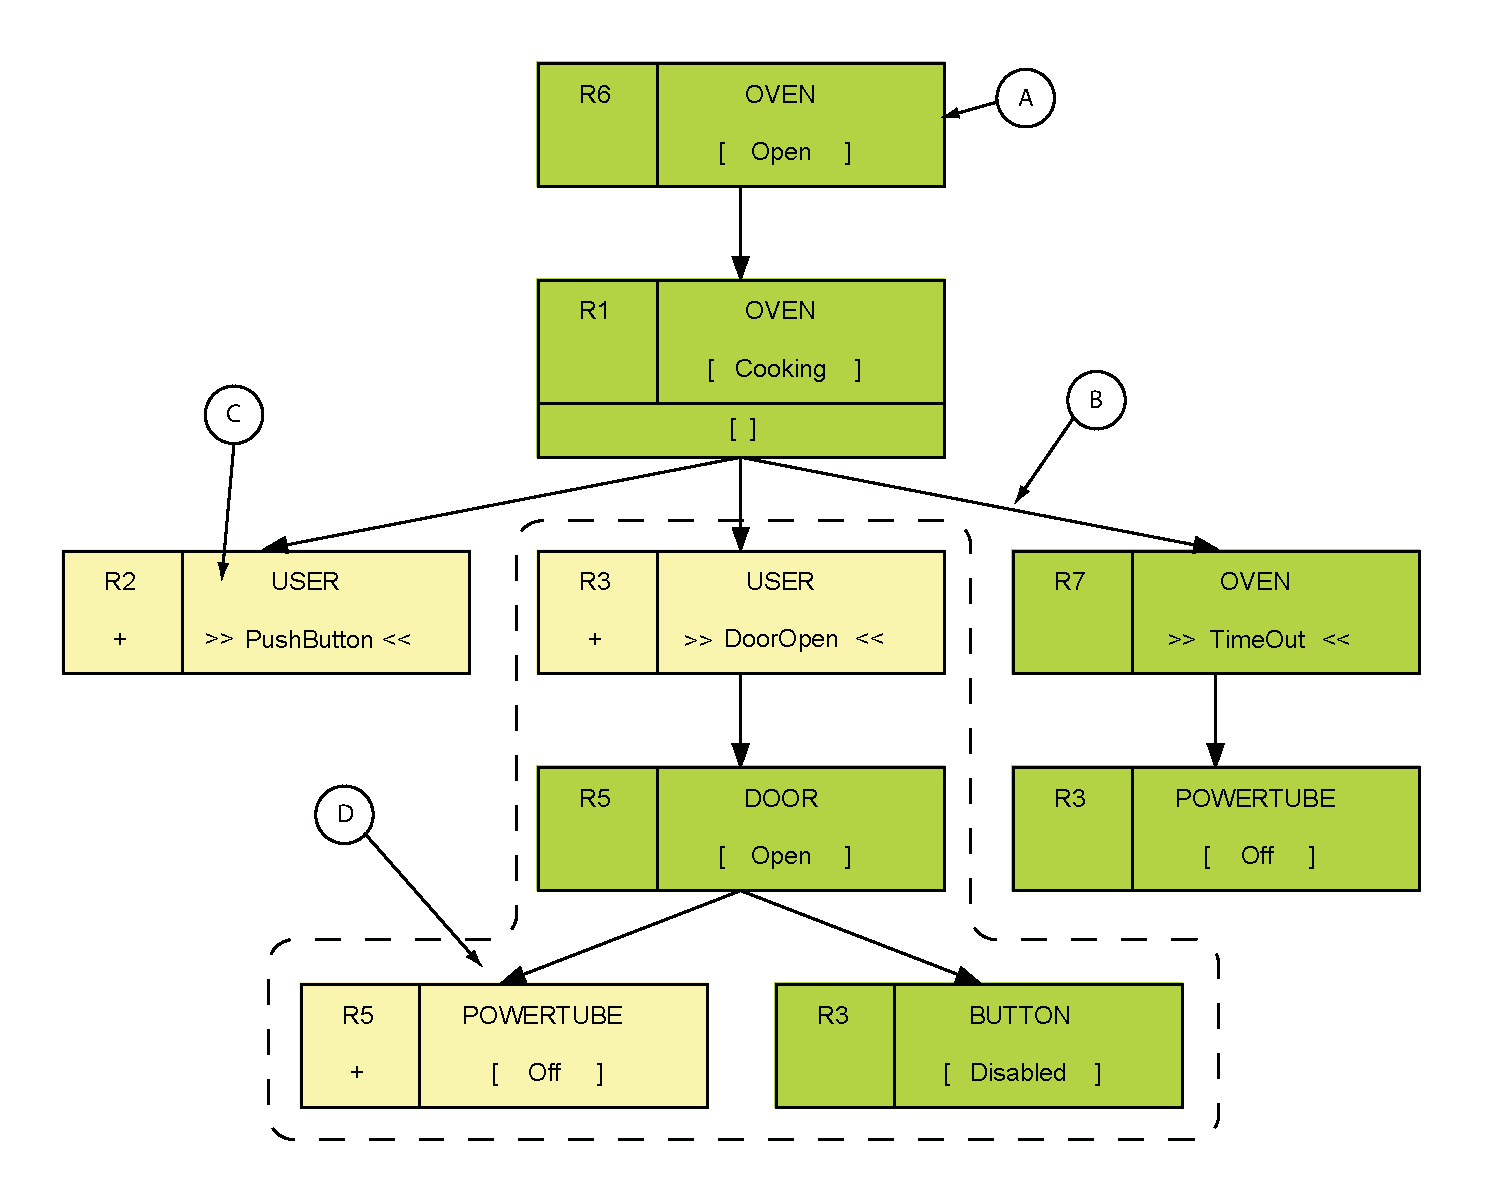
\includegraphics{figs/AppendixB/Naming/Fig3}
 \caption{Tree Branch Naming Convention}
 \label{fig:Naming3}
\end{figure}

\section{Behavior Tree Notation \& Syntax}

\subsection{Node Tags}

\begin{tabularx}{\textwidth}{|c|c|X|}
\textbf{Type} & \textbf{Graphical Notation} & \textbf{Description}\\ \hline
Original &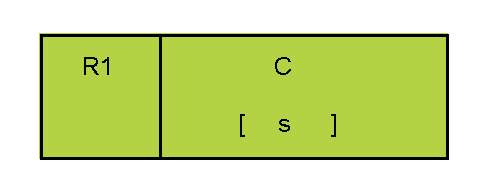
\includegraphics{figs/AppendixB/Tags/Original} & No traceability status indicates that the behavior is stated in the original requirements. The color ``green'' is used for original requirements.\\ \hline
Implied & 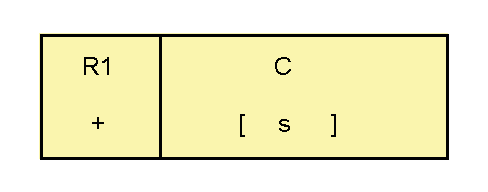
\includegraphics{figs/AppendixB/Tags/Implied} & The ``+'' traceability status indicates that the behavior is not explicitly stated in the original requirements but is implied by the requirement. The color ``yellow'' is used for implied behavior.\\ \hline
Missing &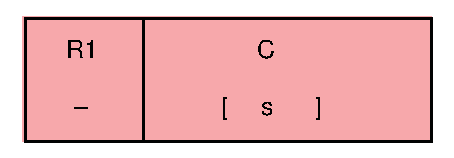
\includegraphics{figs/AppendixB/Tags/Missing}  & The ``-'' traceability status indicates that the behavior is missing from the original requirements and is needed for completeness. The color ``red'' is used for missing behavior.\\ \hline
Design &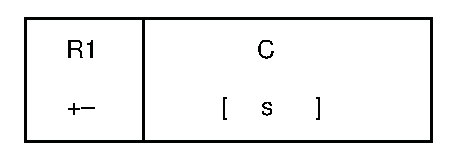
\includegraphics{figs/AppendixB/Tags/Updated} & The ``+-'' traceability
status indicates that the behavior is a refinement of the original requirements, indicating that the behavior is implied but the detail to describe it is missing.\\ \hline
Updated &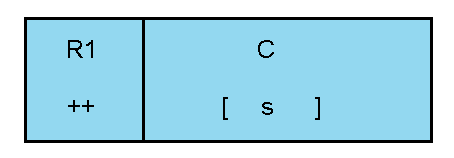
\includegraphics{figs/AppendixB/Tags/Refinement}  & The ``++' traceability status indicates that the behavior has been added in the post-development or maintainence phase. The color ``blue'' is used for updated behavior. Where there are different series of changes / upgrades we use ++v1.0, ++v2.0, etc to indicate the particular upgrade series.\\ \hline
Deleted & 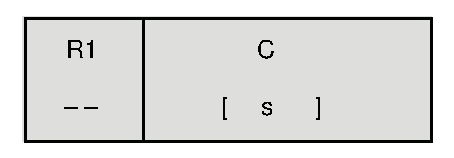
\includegraphics{figs/AppendixB/Tags/Deleted} & The ``--'' traceability status indicates that the behavior has been deleted from the behavior tree. The color ``grey'' is used for deleted behavior, but the nodes may also be hidden optionally by using tool support.
\end{tabularx}

\subsection{Basic Nodes}

\begin{tabularx}{\textwidth}{|c|c|X|}
\textbf{Type} & \textbf{Graphical Notation} & \textbf{Description}\\ \hline
State Realisation &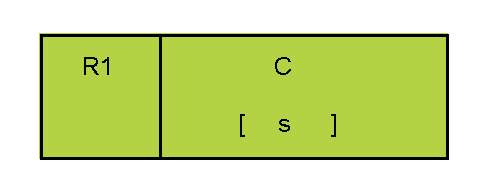
\includegraphics{figs/AppendixB/BasicNodes/StateRealisation} & Component C realises state s.\\ \hline
System State Realisation &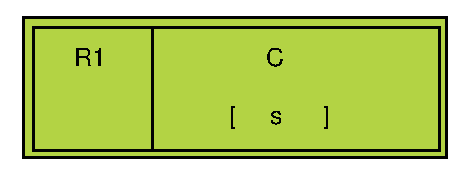
\includegraphics{figs/AppendixB/BasicNodes/SystemStateRealisation}& This is a state realisation decorated with a double box to indicate the component is a system component in the current context. There can only be one system component in each context.\\ \hline
Selection &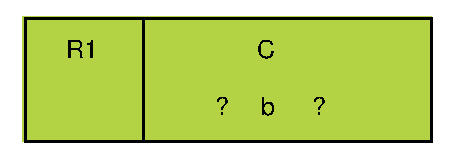
\includegraphics{figs/AppendixB/BasicNodes/Selection} & If condition $b$ evaluates to true, then pass control to child nodes otherwise terminate.\\ \hline
Event &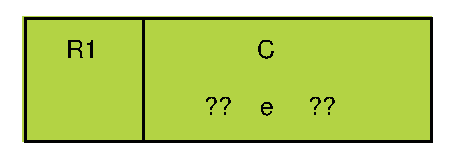
\includegraphics{figs/AppendixB/BasicNodes/Event} & Wait until event $e$ is received.\\ \hline
Guard &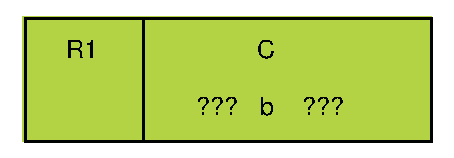
\includegraphics{figs/AppendixB/BasicNodes/Guard} & Wait until condition $b$ evaluates to true, then pass control to child nodes.\\ \hline
Internal Output &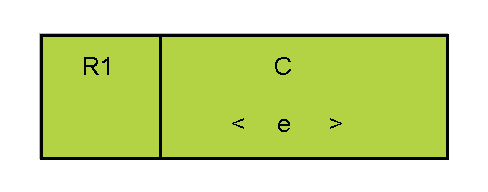
\includegraphics{figs/AppendixB/BasicNodes/IOEvent}  & Generate input $e$ and send to the system.\\ \hline
Internal Input &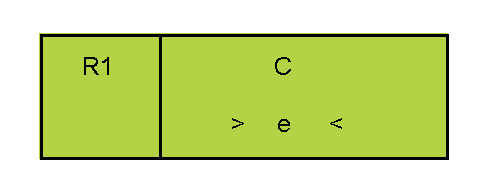
\includegraphics{figs/AppendixB/BasicNodes/IIEvent} & Wait for input $e$ from the system.\\ \hline
External Output &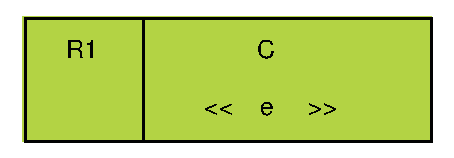
\includegraphics{figs/AppendixB/BasicNodes/EOEvent} & Generate output $e$ and send to the environment.\\ \hline
External Input &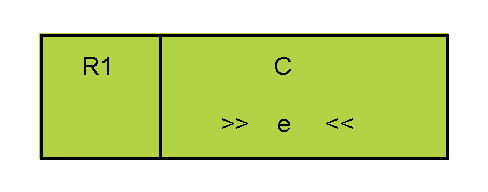
\includegraphics{figs/AppendixB/BasicNodes/EIEvent} & Wait for
input $e$ to be received from the environment.\\ \hline
Empty Node&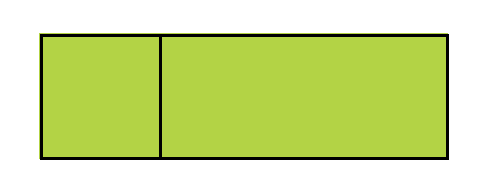
\includegraphics{figs/AppendixB/BasicNodes/Empty} & Empty Nodes can be used together with labels to be origins or destinations of node operators. Empty Nodes are also useful for grouping child nodes into multiple branch types.
\end{tabularx}

\subsection{Behavior Tree Composition}

\begin{tabularx}{\textwidth}{|c|c|X|} 
\textbf{Type} & \textbf{Graphical Notation} &  \textbf{Description}\\ \hline
Sequential Composition&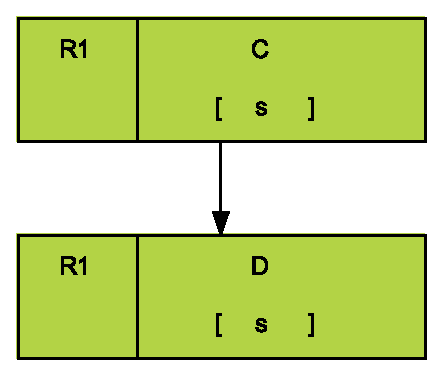
\includegraphics{figs/AppendixB/Composition/Sequential} &Execute $N$, passing control to tree $T$. The behavior of concurrent BTs may be interleaved between $N$ and $T$.\\ \hline
Atomic Composition&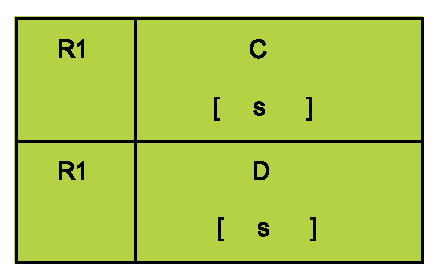
\includegraphics{figs/AppendixB/Composition/Atomic} & Execute $N_1$ immediately followed by $N_2$, passing control to tree $T$. The behavior of concurrent BTs may not be interleaved between $N_1$ and $N_2$.\\ \hline
Parallel Branching&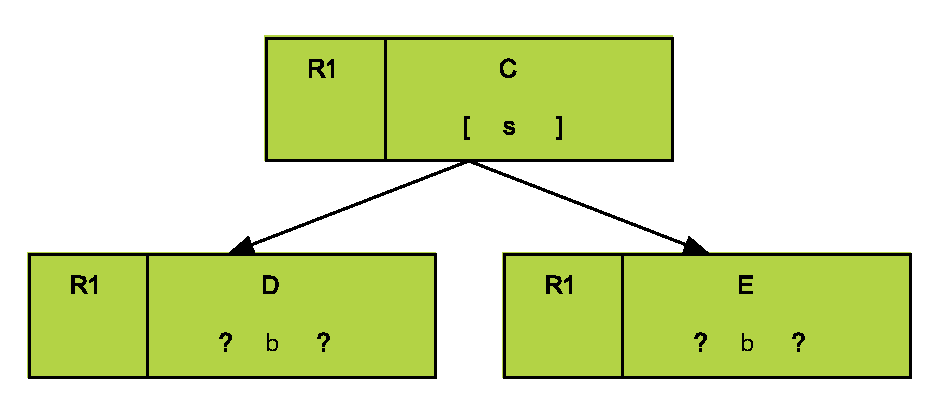
\includegraphics{figs/AppendixB/Composition/Parallel} &  Execute $N$, passing control to both $T_1$ and $T_2$.\\ \hline
Alternative Branching&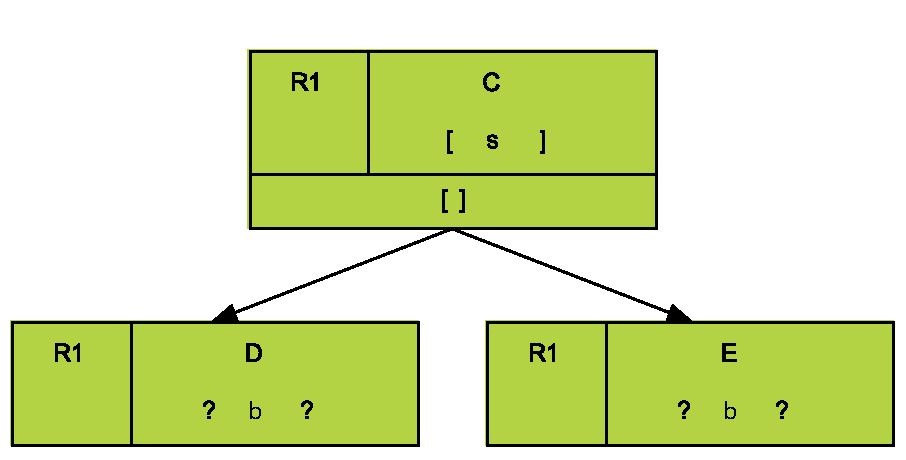
\includegraphics{figs/AppendixB/Composition/Alternative}& 
A nondeterministic choice is made between $T_1$ and $T_2$, depending on which is ready to execute (not blocked)
\end{tabularx}


\subsection{Node Operators}
\begin{itemize}
\item Operators on source nodes match against the Component, Behavior, Behavior Type and Label (if present) of the destination node.
\item An operator may be prefixed by a label and a fullstop to refer to a destination node with a label e.g. $lbl.^{\wedge}$ indicates to revert to destination node with label $lbl$.
\end{itemize}

\begin{tabularx}{\textwidth}{|c|c|X|}
\textbf{Type} & \textbf{Graphical Notation} & \textbf{Description}\\ \hline 
Reference &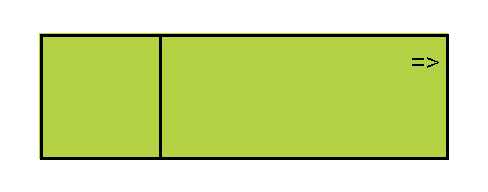
\includegraphics{figs/AppendixB/Operators/Reference} & Behave as the destination node. The destination node must appear in an alternative branch to the origin.\\ \hline
Reversion &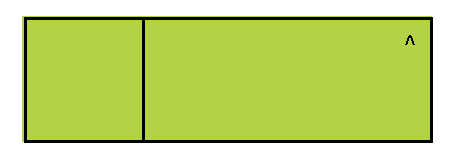
\includegraphics{figs/AppendixB/Operators/Reversion} & Behave as the destination node. The destination node must be an ancestor. All sibling behaviour is terminated.\\ \hline
Branch Kill &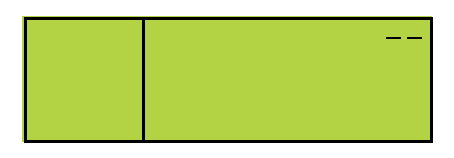
\includegraphics{figs/AppendixB/Operators/BranchKill} & Terminate all behavior associated with destination tree.\\ \hline
Synchronisation &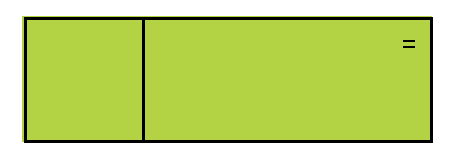
\includegraphics{figs/AppendixB/Operators/Synchronisation} & Wait for destination node (or nodes).\\ \hline
May &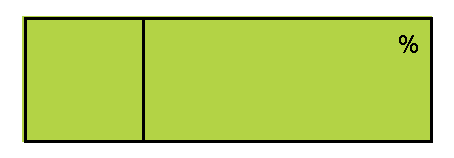
\includegraphics{figs/AppendixB/Operators/May} & The node may execute normally, or may have no effect.\\ \hline
Conjunction &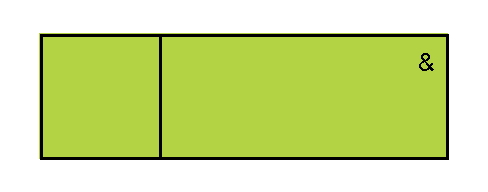
\includegraphics{figs/AppendixB/Operators/Conjunction} & The operators \&, $|$ and $XOR$ correspond to logical conjunction, disjunction and exclusive or respectively.\\ 
 \cline{1-2}
Disjunction &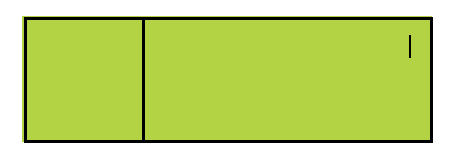
\includegraphics{figs/AppendixB/Operators/Disjunction} &\\
 \cline{1-2}
Exclusive OR &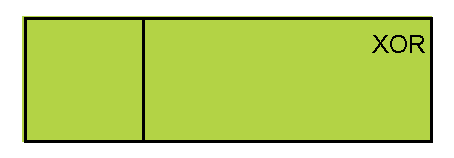
\includegraphics{figs/AppendixB/Operators/XOR} &
\end{tabularx}



\end{document}